\section{Plugin Eclipse}

Per il progetto è stato sviluppato un plugin per Eclipse che si occupa di:
\begin{itemize}
  \item text-highlight
  \item controllo degli errori
  \item compilazione
\end{itemize} 

Il pacchetto viene fornito sia come archivio (da estrarre nella cartella di un
eclipse) sia come IDE completo basato sul platform di Eclipse 3.2 (Callisto).

\begin{figure}[htp]
\begin{center}
  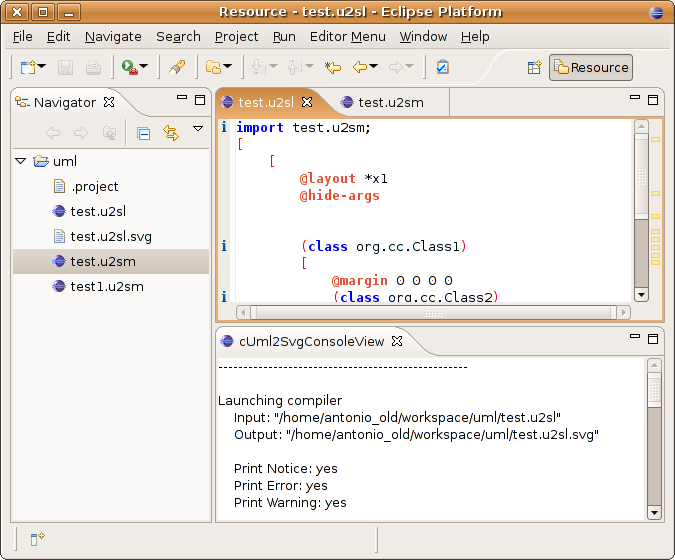
\includegraphics[width=0.9\textwidth]{img/eclipse}
  \caption[labelInTOC]{Screenshot dell'ambiente eclipse con un editor di layout
  attivo}
  \label{errorieditor} 
\end{center}
\end{figure}


\subsection{Text-highlight}
Il plugin gestisce il \emph{modello dati} e lo \emph{schema di layout} in modi differenti; 
entrambi, infatti, presentano caratteristiche e strutture diverse tra loro. 
La classe che esegue la scansione del \emph{modello dati} e ne gestisce l'editor
è la ``ModelScanner'' di cui vediamo i passi essenziali:

In questo spezzone di codice vengono definite le keyword del file di tipo modello:
\begin{lstlisting}[caption={ModelScanner}, style={java}]
	private static String[] keywords= { "class","package", "public",
			"private","interface", "methods","extend", "relations", 
			"attributes"  };
\end{lstlisting}

Vengono poi definite (nel Costruttore) una lista di regole che definiscono cosa
evidenziare associandole a un ``token'' che definisce l'aspetto:

\begin{lstlisting}[caption={ModelScanner}, style={java}]
	public ModelScanner(ColorManager manager) {
					manager.getColor(ColorConstants.DEFAULT)));
		ArrayList<IRule> rules= new ArrayList<IRule>();	
		Token tokencomment = new Token(new TextAttribute(
						manager.getColor(ColorConstants.COMMENT)));
		//Add rule for processing instructions
		rules.add( new SingleLineRule("//", "\n", tokencomment));
		rules.add( new SingleLineRule("#", "\n", tokencomment));
		rules.add( new MultiLineRule("/*", "*/", tokencomment));
		
		Token token= new Token(new TextAttribute(
				manager.getColor(ColorConstants.KEYWORD), 	//parola
				null,                                       //sfondo
				SWT.BOLD));
		WordRule wordRule = new WordRule(new WordDetector());
		for (int i = 0; i < keywords.length; i++) {
			wordRule.addWord(keywords[i], token);
		}		
		rules.add(wordRule);
		
		token = new Token(new TextAttribute(
							manager.getColor(ColorConstants.BRACET)));
		RuleBrace braceRule = new RuleBrace(token);
		rules.add(braceRule);
		
		IRule[] r= new IRule[rules.size()];
		setRules(rules.toArray(r));
	}
}
\end{lstlisting}

La classe che esegue la scansione dello  \emph{schema di layout} e ne gestisce
l'editor, ha la stessa struttura di quella del \emph{modello dati}; le regole
per i commenti e per le parentesi, infatti, non cambiano. 
L'unica differenza è nella gestione delle keywords che nel modello dello
\emph{schema di layout} si presenta così:

\begin{lstlisting}[caption={LayoutScanner}, style={java}]
	private static String[] keywordslayout= {"@layout","@hide-args",
												"@collapse","@margin"};
	private static String[] keywords= { "class","import","interface"};
	
	public LayoutScanner(ColorManager manager) {
		ArrayList<IRule> rules= new ArrayList<IRule>();
		Token token= new Token(new TextAttribute(
				manager.getColor(ColorConstants.KEYWORD), 	//parola
				null,                                       //sfondo
				SWT.BOLD));
		Token tokenlayout= new Token(new TextAttribute(
				manager.getColor(ColorConstants.LAYOUT), 	//parola
				null,                                     //sfondo
				SWT.BOLD));
		
\end{lstlisting}

La divisione delle parole chiave, che sono specificate nella stringa 
\emph{Keywords} e delle proprietà dello schema, che sono specificate nella
stringa \emph{keywordslayout},  è stata fatta per dare la possibilità 
di gestirle in modo separato.


\subsection{Controllo degli errori} 

Il plugin si occupa di visualizzare, tramite dei marker laterali, gli errori 
commessi in fase di scrittura del \emph{modello dati} e dello \emph{schema di
layout}.
Il controllo degli errori viene eseguito ogni volta che il file su cui si stà lavorando
viene salvato; 
Vengono controllati tutti i tipi di errori:
\begin{itemize}
  \item errori semantici
  \item errori sintattici
  \item erorri lessicali
\end{itemize} 

Vengono inoltre gestiti tutti i messaggi di attenzione (Warning) e nitifica
(Notice) segnalandoli con icone opportune

La classe che si occupa della gestione dei marker è la seguente
``AbstractCompilerMessageParser'' che prende in input i messaggi prodotti dal
compilatore ed effettuando il parsing riga per riga estrae i messaggi validi e
li adatta al codice sorgente in base al tipo e alla linea che ha generato l'errore.



\begin{figure}[htp]
\begin{center}
  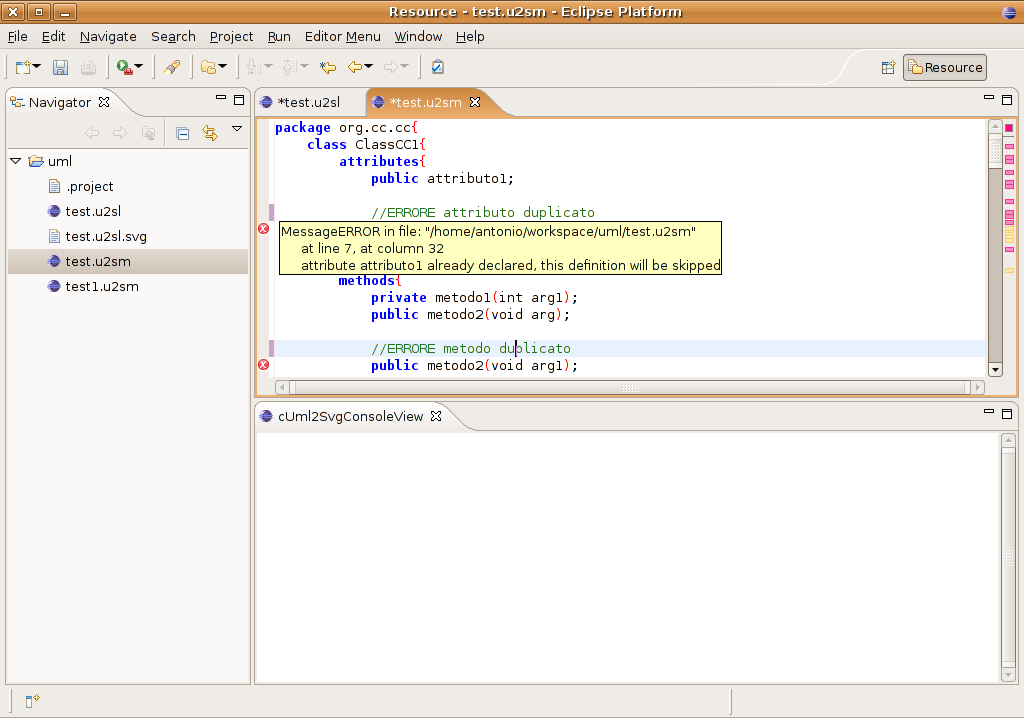
\includegraphics[width=0.9\textwidth]{img/error}
  \caption[labelInTOC]{Esempio di segnalazione di errore}
  \label{errorieditor} 
\end{center}
\end{figure}

\begin{figure}[htp]
\begin{center}
  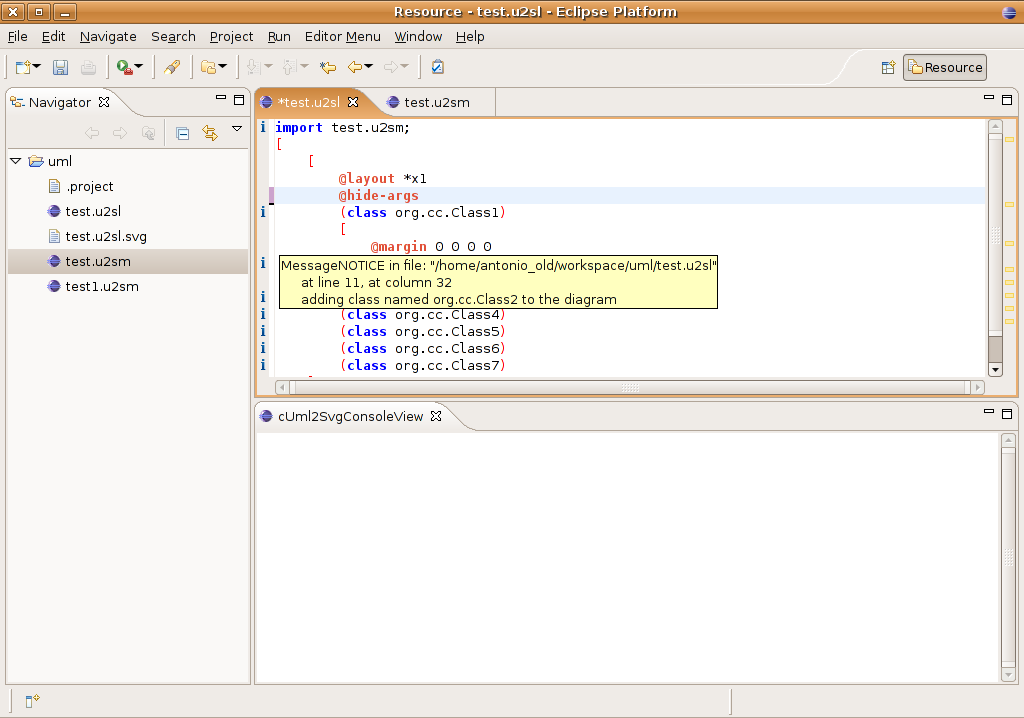
\includegraphics[width=0.9\textwidth]{img/notice}
  \caption[labelInTOC]{Esempio di segnalazione di notifica}
  \label{errorieditor} 
\end{center}
\end{figure}
 
 \subsection{Compilazione} 
La compilazione avviene in modo implicito nel momento del salvataggio di un file
di tipo layout. Così facendo viene permesso allo sviluppatore di correggere alcuni
errori ancor prima di visualizzare l'output di compilazione.

Il file compilato per default è un file con il nome del file di layout seguito
dall'estenzione ``.svg''.

E' stata pure sviluppata una ``Vista Console'' per visualizzare tutto l'output
generato dal plugin.

\begin{figure}[htp]
\begin{center}
  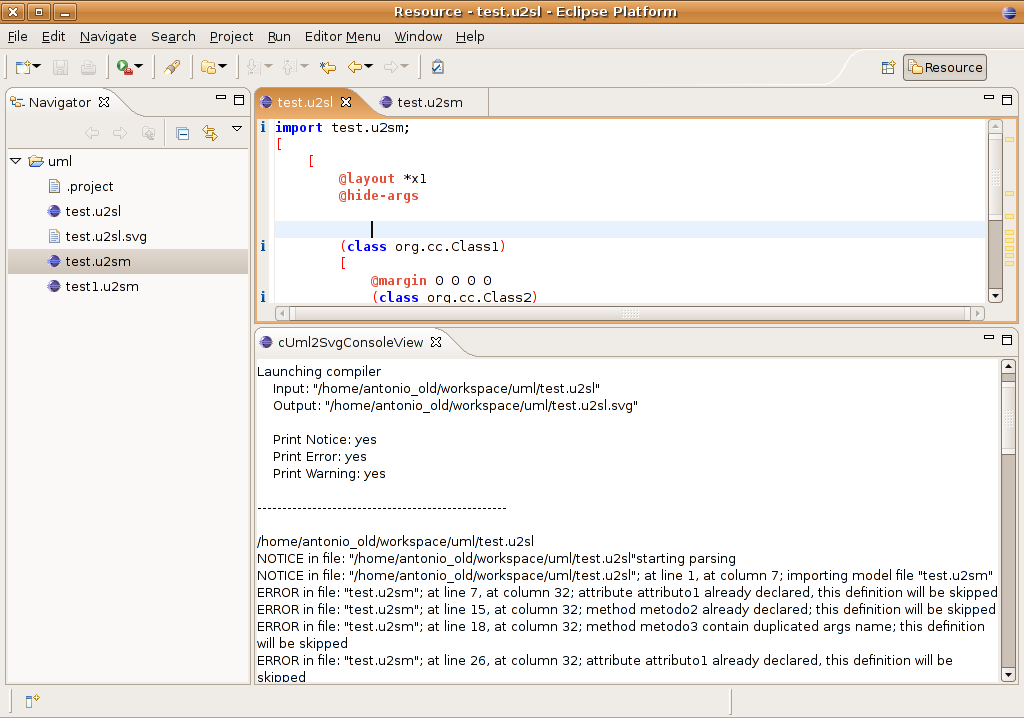
\includegraphics[width=0.9\textwidth]{img/console_view}
  \caption[labelInTOC]{Vista Console}
  \label{errorieditor} 
\end{center}
\end{figure}